\chapter{Análisis}


\section{Arquitectura Modelo-Vista-Controlador}

Para el cumplimiento del requisito de la escalabilidad del chatbot, un paso a seguir es conseguir un bajo acoplamiento entre las partes del sistema. Teniendo en cuenta el sistema que se va a desarrollar, un patrón de diseño de arquitectura que se ajusta muy bien a él es la arquitectura Modelo-Vista-Controlador (MVC). Esta arquitectura se compone de las siguientes elementos:

\begin{itemize}
    \item Modelo
    \item Vista
    \item Controlador
\end{itemize}

Teniendo cada una de estas partes una funcionalidad clara y en gran medida independiente del resto. 

Las principales ventajas de esta arquitectura son las siguientes:

\begin{itemize}
    \item Permite la programación paralela e independiente de cada una de las partes de la arquitectura
    \item Independencia en el funcionamiento de las partes
    \item Facilita la gestión de errores al ser tan modular el sistema, dado que los errores estarán más aislados y se podrán abordar de forma más eficiente, y por supuesto también porque se pueden sustituir esos módulos con errores por otros en buen estado.
    \item Facilita la escalabilidad del sistema al poder conectar nuevos módulos de cada una de las partes de la arquitectura, sin tener que modificar el resto de partes
    \item Permite una importante separación entre los datos y su representación visual
\end{itemize}

Pero todas estas ventajas tienen un coste que hay que asumir, y este coste es principalmente un aumento de complejidad en todos los ámbitos, por un lado provoca un aumento de la cantidad de código necesaria, este aumento de código implica tener un mayor número de archivos que mantener, y por último dificulta la curva de aprendizaje del sistema.

A continuación se mostrará una breve definición de cada una de estas partes, basándome en un artículo de revista sobre la arquitectura (referencia a Capítulo II. Arquitectura del Software).

\subsection*{Vista}

La Vista es el objeto que maneja la presentación visual de los datos representados por el Modelo, es decir, es la capa sobre la que se muestran los resultados esperados por el usuario y con la que realiza la interacción el usuario.

\subsection*{Controlador}

El Controlador es el objeto que proporciona significado a las órdenes del usuario, actuando sobre los datos representados por el Modelo, centra toda la interacción entre la Vista y el Modelo, es decir, es la capa encarga de centralizar todas las conexiones entre el resto de capas, manejando las entradas, transfiriendo las al modelo de forma correcta y devolviendo la respuesta del Modelo a la Vista. Además es el encargado de modificar el Modelo en caso de que sea necesario.

\subsection*{Modelo}

El Modelo es el objeto que representa la información del programa. Maneja los datos y controla todas sus transformaciones, es decir, contiene y maneja toda la información del sistema salvo el conocimiento específico del Controlador ó de la Vista.

\subsection{Ciclo de vida de MVC}

Las conexiones entre las distintas partes están muy bien definidas y acotadas para tener un bajo acoplamiento.

El Controlador recibe las entradas del usuario, el Controlador transmite la peticiones al Modelo, el cuál realiza las tareas de la petición y devuelve el resultado al Controlador, y este a su vez devuelve la respuesta a la Vista para que el usuario pueda observar los resultados de su entrada.

\begin{figure}[h]
    \centering
    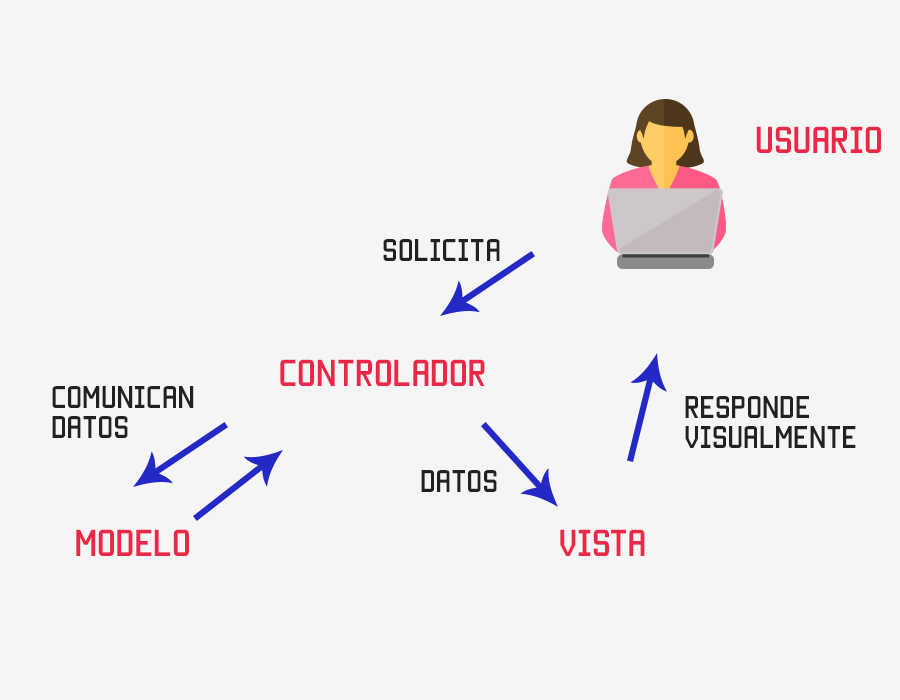
\includegraphics[width=0.8\textwidth]{imagenes/04_Analisis/ciclo_vida_MVC.jpg}
    \begin{center}
        (Fuente: \url{https://codigofacilito.com/articulos/mvc-model-view-controller-explicado})
    \end{center}
    \caption{Ciclo de vida de MVC}
\end{figure}

\subsection{Adaptación del proyecto a la arquitectura}


